\documentclass[11pt,a4paper,openany]{report}

\usepackage[T1]{fontenc}
\usepackage{lmodern}
\usepackage{microtype}
\usepackage{amsmath,amssymb,amsthm,mathtools,bm}
\usepackage{booktabs,array,longtable,tabularx}
\usepackage{xcolor}
\usepackage[margin=24mm,headheight=23pt]{geometry}
\usepackage{enumitem}
\usepackage{fancyhdr}
\usepackage{fancyvrb}
\usepackage{graphicx}
\usepackage{url}
\usepackage{hyperref}

\definecolor{finblue}{HTML}{1F5A99}
\definecolor{fingreen}{HTML}{19733A}
\definecolor{finorange}{HTML}{D55E00}
\definecolor{finred}{HTML}{A61B1B}
\definecolor{finviolet}{HTML}{6A3D9A}
\definecolor{fingray}{HTML}{4D4D4D}

\hypersetup{
  unicode=true,
  colorlinks=true,
  linkcolor=finblue,
  citecolor=fingreen,
  urlcolor=finblue,
  pdftitle={FIN Reconstructed Legacy Kernel: Programs 41--50},
  pdfauthor={Krzysztof \.Zuchowski},
  pdfsubject={Program 42a methodology audit and Programs 41--50 on K^*_legacy},
  pdfkeywords={FIN, legacy kernel, dual dynamics, selector, units, Programs 41-50}
}

\pagestyle{fancy}
\fancyhf{}
\fancyhead[L]{\small FIN Reconstructed Legacy Kernel}
\fancyhead[R]{\small Release 10.4}
\fancyfoot[C]{\thepage}
\setlength{\parindent}{0pt}
\setlength{\parskip}{0.55em}
\setlist{nosep,leftmargin=2em}
\setcounter{tocdepth}{2}
\setcounter{secnumdepth}{3}
\emergencystretch=2em

\newcommand{\one}{\bm 1}
\newcommand{\C}{\mathbb C}
\newcommand{\R}{\mathbb R}
\newcommand{\Z}{\mathbb Z}
\newcommand{\statusProven}{\textcolor{fingreen}{[Proven]}}
\newcommand{\statusStrong}{\textcolor{finblue}{[Strong evidence]}}
\newcommand{\statusModerate}{\textcolor{finviolet}{[Moderate evidence]}}
\newcommand{\statusWeak}{\textcolor{fingray}{[Weak evidence]}}
\newcommand{\statusSpeculative}{\textcolor{finorange}{[Speculative]}}
\newcommand{\statusRefuted}{\textcolor{finred}{[Refuted]}}

\begin{document}
\hypersetup{pageanchor=false}
\begin{titlepage}
\centering
\vspace*{10mm}
{\Large\bfseries FIN Research Supplement --- Release 10.4\par}
\vspace{11mm}
{\Huge\bfseries FIN Reconstructed Legacy Kernel\par}
\vspace{6mm}
{\Large Program 42a Methodology Audit and Executed Programs 41--50 on \(K^*_{\mathrm{legacy}}\)\par}
\vspace{17mm}
{\Large Krzysztof \.Zuchowski\par}
\vspace{2mm}
{\normalsize Independent Researcher --- Fractal Information Theory Project\par}
\vspace{2mm}
{\normalsize ORCID: \href{https://orcid.org/0009-0002-0909-3613}{0009-0002-0909-3613}\par}
\vspace{10mm}
{\large 19 July 2026\par}
{\normalsize Publication --- Preprint; record version 1.0.0\par}
\vfill
\begin{minipage}{0.88\textwidth}
\small
\textbf{Scope.} Algebraic reconstruction of the historical legacy kernel, rejection of a double-damped product candidate, dual-dynamics audits, and ten executed programs (41--50) on the corrected class \(K^*\).

\medskip
\textbf{Guardrail.} No silent legacy--strict identification, no role transfer, no selector closure, no physical unit export, no Theory-of-Everything claim.

\medskip
\textbf{Reproducibility.} \path{fin_programs_41_50_legacy_star.py}, \path{FIN_Programs_41_50_Legacy_Star_Results.json}, figures, Markdown, LaTeX.

\medskip
\textbf{License.} Creative Commons Attribution 4.0 International (CC BY 4.0).
\end{minipage}
\vfill
\end{titlepage}
\hypersetup{pageanchor=true}

\pagenumbering{roman}
\chapter*{Publication statement}
\addcontentsline{toc}{chapter}{Publication statement}
This preprint freezes the path-transformed reconstructed legacy class
\[
K^*_{\mathrm{legacy}}(d)=A\frac{\cos(\pi d/4+\pi/6)}{1+\beta d}
\]
after Program~42a, executes Programs~41--50, and records that units, selector, and symmetry-breaking leaf-cuts remain open under current artifacts.

\tableofcontents
\clearpage
\pagenumbering{arabic}

\section{Confidence convention}

\begin{itemize}
\item 
\textbf{\statusProven{}} analytic proof or exact finite algebra under stated definitions.

\item 
\textbf{\statusStrong{}} reproducible numerical result with wide margin, not a general theorem.

\item 
\textbf{\statusModerate{}} model-dependent or limited alternative class.

\item 
\textbf{\statusSpeculative{}} admissible construction without source theorem.

\item 
\textbf{\statusRefuted{}} obstruction or explicit counterexample in the stated scope.

\end{itemize}

All times, rates, couplings, and kernel values below are dimensionless. No SI unit, physical clock, non-premise selector, legacy role transfer, or Theory-of-Everything claim is exported.

\par\medskip\hrule\medskip

\chapter{Executive summary}

This monograph does three things.

\begin{enumerate}
\item 
It audits the Program 42a algebraic reconstruction of the historical legacy kernel against DIAGRAMS\_KERNEL\_TRANSFORMATION.md and against a cheap dual-dynamics reading of a proposed product formula.

\item 
It freezes the algebraically corrected class \[
   K^*_{\mathrm{legacy}}(d)
   =
   A\,\frac{\cos(\pi d/4+\pi/6)}{1+\beta d}
   \] and runs the ten research programs recommended after Programs 31–40.

\item 
It answers, under AGENTS.md /\allowbreak{} SUMMARY\_GROK.md guardrails, whether the new kernel dissolves the three leaf-cuts: dimensionlessness, selector /\allowbreak{} QW-2191, and symmetry breaking.

\end{enumerate}

\textbf{Main verdicts.}

\begin{itemize}
\item 
\textbf{\statusRefuted{}} The product candidate \[
  K_{\mathrm{rej}}(d)
  =
  e^{-2.9d}\,\frac{1+0.2d}{1+d}\,
  \cos\!\Bigl(\frac{\pi d}{4}+\frac{\pi}{6}\Bigr)
  \] is not a faithful historical reconstruction: it swaps resonance/\allowbreak{}torsion roles, double-counts damping, fails the corrected path-sum asymptotics, and kills inverse hierarchy.

\item 
\textbf{\statusProven{}} After path-sum algebra, the historically intended effective class is the hyperbolic-phase form \(K^*\) above. Parameters \(A,\beta\) are not uniquely fixed by the diagram alone.

\item 
\textbf{\statusStrong{}} After absolute-value positivity repair on \(\mathbb Z_{12}\), \(K^*\) supports dual dynamics: unitary \(U_t=e^{-itA}\) and Markov \(P_t=e^{-tA}\) with \(A=sI-W\).

\item 
\textbf{\statusProven{}} Dual dynamics does \textbf{not} export units, a non-premise selector, or orientation breaking. The three leaf-cuts remain open.

\item 
\textbf{\statusProven{}} Programs 41–50 show: Loewner bridge is support/\allowbreak{}normalization dependent; affine phase maps leave envelope residual; hazard laws do not hold out; Markov relative information is monotone while unitary Born information is not; environment dilation can hold lost information; external polarity is apparatus-level only; multi-size cosine challenge selects the strict profile when it is among competitors.

\end{itemize}

Honest conclusion:

\begin{quote}\itshape
\(K^*_{\mathrm{legacy}}\) is a better intermediate historical object than the double-damped product, and a usable dual-dynamics generator after positivity repair. It is \textbf{not} a free lunch for units, selector, or ToE.

\end{quote}

\par\medskip\hrule\medskip

\chapter{Part I — Program 42a methodology audit}

\section{1. Input axioms (reconstruction only)}

From DIAGRAMS\_KERNEL\_TRANSFORMATION.md:

\[
K_{\mathrm{total}}
=
K_{\mathrm{geo}}\,K_{\mathrm{res}}\,(1+0.2\,K_{\mathrm{tors}})\,K_{\mathrm{topo}}.
\]

Historical role assignment:

\begin{center}
\begingroup\small
\setlength{\tabcolsep}{3.5pt}
\renewcommand{\arraystretch}{1.16}
\begin{longtable}{@{}p{0.217\textwidth}p{0.316\textwidth}p{0.327\textwidth}@{}}
\toprule
\textbf{Factor} & \textbf{Historical meaning} & \textbf{Diagram form} \\
\midrule
\endhead
\(K_{\mathrm{geo}}\) & viscosity /\allowbreak{} catastrophic damping & \(e^{-2.9d}\) \\
\(K_{\mathrm{res}}\) & resonance /\allowbreak{} phase sync & \(\approx 0.8\)–\(1.2\) \\
\(K_{\mathrm{tors}}\) & turbulent currents & \(\cos(\pi d/4+\pi/6)\) \\
\(K_{\mathrm{topo}}\) & topology /\allowbreak{} path sum & \(\to 1/(1+\beta d)\) after transform \\
\bottomrule
\end{longtable}
\endgroup
\end{center}

Section 8 of the diagram states that exponential viscosity is \textbf{transformed} into hyperbolic damping by fractal path summation, not multiplied by it again.

\section{2. Audit errors A/\allowbreak{}B/\allowbreak{}C}

\subsection{(A) Exponential damping}

\textbf{\statusProven{}} The viscosity rate \(2.9\) must be used exactly when \(K_{\mathrm{geo}}\) is written. The rejected product does use \(e^{-2.9d}\), so (A) alone is not its fatal flaw. Its flaw is combining that exponential with a second damping factor.

\subsection{(B) Path scaling}

If \(N(d)\sim d^{1.6}\) and one wants total contribution \(\sim d^{-1}\) (large-\(d\) tail of \(1/(1+\beta d)\)), then

\[
A_{\mathrm{path}}(d)\sim d^{-2.6}.
\]

The diagram’s \(A_{\mathrm{path}}\sim d^{-0.6}\) would give \(N A\sim d^{1.0}\) (growth), not a decaying hyperbolic tail. \textbf{\statusProven{}}

\subsection{(C) Exact phase zeros}

\[
\cos\Bigl(\frac{\pi d}{4}+\frac{\pi}{6}\Bigr)=0
\quad\Longleftrightarrow\quad
d=\frac43+4n.
\]

Zeros are \(d=1.333,5.333,9.333,\ldots\), not the integer sequence \(2,5,8,11\). Cosine values at those integers are nonzero (e.g. \(\cos(\pi/2+\pi/6)=-1/2\) at \(d=2\)). \textbf{\statusProven{}}

\section{3. Rejection of the product candidate}

The proposed assignment

\[
K_{\mathrm{geo}}=e^{-2.9d},\quad
K_{\mathrm{res}}=\cos(\cdot),\quad
K_{\mathrm{tors}}=d,\quad
K_{\mathrm{topo}}=1/(1+d)
\]

fails diagram fidelity on four counts:

\begin{enumerate}
\item 
resonance and torsion roles are swapped;

\item 
\(K_{\mathrm{tors}}=d\) is not the historical oscillatory current;

\item 
\(e^{-2.9d}\times 1/(1+d)\) double-counts damping against §8;

\item 
\((1+0.2d)/(1+d)\to 0.2\) is asymptotically constant, not a \(1/d\) path-sum tail.

\end{enumerate}

Numerical profile on \(d=1..12\): \(|K_{\mathrm{rej}}|\) falls below \(10^{-3}\) by \(d=2\) and is numerically dead thereafter. Correlation with classical frozen legacy is only \(\approx 0.21\). \textbf{\statusStrong{}}

\textbf{Verdict on product form:} \textbf{odrzucona} (confidence \(\approx 25/100\) as historical reconstruction).

\section{4. Accepted reconstructed class}

After path-sum correction:

\[
\boxed{
K^*_{\mathrm{legacy}}(d)
=
A\,\frac{\cos(\pi d/4+\pi/6)}{1+\beta d}
}
\]

with free positive scales \(A,\beta\). Historical diagram ranges suggest \(\beta\in[0.01,0.08]\) and amplitude near \(2.7\)–\(3.0\). Freezes used in this report:

\begin{center}
\begingroup\small
\setlength{\tabcolsep}{3.5pt}
\renewcommand{\arraystretch}{1.16}
\begin{longtable}{@{}p{0.229\textwidth}p{0.149\textwidth}p{0.170\textwidth}p{0.312\textwidth}@{}}
\toprule
\textbf{Freeze} & \textbf{\(A\)} & \textbf{\(\beta\)} & \textbf{Role} \\
\midrule
\endhead
Historical & \(2.9\) & \(0.05\) & diagram-scale intermediate \\
\(\mathbb Z_{12}\) & \(1\) & \(1\) & unitless Laplacian scale \\
Classical frozen & \(4\ln 2\) & \(0.01\) & post-hoc comparison only \\
\bottomrule
\end{longtable}
\endgroup
\end{center}

\textbf{\statusProven{}} Reconstruction did not use \(K_{\mathrm{strict}}\) to choose the functional form.\\
\textbf{\statusProven{}} The operator is \textbf{not} unique: only the class is.

\section{5. Cheap dual-dynamics reading}

The cheap analysis correctly notes that any real self-adjoint generator \(A\) supports both \(e^{-itA}\) and \(e^{-tA}\). It incorrectly treats the product form as historically faithful and as automatically Markov-stable. Signed weights on \(\mathbb Z_{12}\) are not all nonnegative; absolute-value repair is an extra declaration. Dual dynamics after repair does \textbf{not} validate the rejected product algebra.

\par\medskip\hrule\medskip

\chapter{\texorpdfstring{Part II — Dual dynamics for \(K^*\)}{Part II — Dual dynamics for K\textasciicircum{}*}}

\section{6. Operator construction}

Sample radial weights on cyclic distances \(d=1,\ldots,6\), set \(W_{xx}=0\), \(W_{xy}=|K^*(d(x,y))|\) (positivity repair), and

\[
A=sI-W,\qquad s=\text{common row sum}.
\]

Then Dirichlet identity holds and \(A\succeq 0\) with simple kernel of constants when all off-diagonal weights are positive. \textbf{\statusProven{}} under the repair declaration.

Selected numerical dual-dynamics rows:

\begin{center}
\begingroup\footnotesize
\setlength{\tabcolsep}{3.5pt}
\renewcommand{\arraystretch}{1.16}
\begin{longtable}{@{}p{0.184\textwidth}p{0.147\textwidth}p{0.162\textwidth}p{0.163\textwidth}p{0.204\textwidth}@{}}
\toprule
\textbf{Object} & \textbf{\(s\)} & \textbf{gap \(\gamma\)} & \textbf{Markov escape \(\sim\)} & \textbf{Unitary short escape proxy} \\
\midrule
\endhead
\(K^*_{\mathrm{hist}}\) abs & \(15.440\) & \(14.179\) & \(15.43\) & \(2.7\times10^{-3}\) \\
\(K^*_{\mathrm{Z12}}\) abs & \(1.579\) & \(1.508\) & \(1.579\) & \(2.7\times10^{-5}\) \\
\(K_{\mathrm{rej}}\) abs & \(0.0186\) & \(0.00313\) & \(0.0186\) & \(1.5\times10^{-8}\) \\
\(K_s\) strict & \(1.660\) & \(0.754\) & \(1.660\) & \(5.4\times10^{-5}\) \\
\bottomrule
\end{longtable}
\endgroup
\end{center}

\textbf{\statusStrong{}} \(K^*_{\mathrm{Z12}}\) is spectrally in the same operational ballpark as strict dual dynamics; the rejected product is almost trivial (tiny \(s\)).

Inversion residual of \(A\) under \(x\mapsto -x\) is \(0\) for all radial objects tested: the generator remains orientation-blind. \textbf{\statusProven{}}

\par\medskip\hrule\medskip

\chapter{Part III — Executed Programs 41–50}

Programs follow the roadmap left by Release 10.3, now evaluated on \(K^*\) rather than only classical frozen legacy.

\section{Program 41 — Loewner bridge support scan}

\textbf{Question.} For which supports/\allowbreak{}normalizations is \(A_s-A_\ell\succeq 0\)?

\textbf{Result.} On \(C_{12}\) and interval \(I_{12}\):

\begin{center}
\begingroup\small
\setlength{\tabcolsep}{3.5pt}
\renewcommand{\arraystretch}{1.16}
\begin{longtable}{@{}p{0.281\textwidth}p{0.372\textwidth}p{0.207\textwidth}@{}}
\toprule
\textbf{Legacy object (abs)} & \textbf{min eig\((A_s-A_\ell)\) on \(C_{12}\)} & \textbf{PSD?} \\
\midrule
\endhead
\(K^*_{\mathrm{hist}}\) & \(-19.715\) & no \\
\(K^*_{\mathrm{Z12}}\) & \(-0.754\) & no \\
classical \(|K_\ell|\) & \(-21.221\) & no \\
rejected abs & \(\approx 0\) & yes (trivial) \\
\bottomrule
\end{longtable}
\endgroup
\end{center}

\textbf{\statusProven{}} Loewner positivity is support- and normalization-dependent. The rejected product looks “PSD-bridgeable” only because its weights are nearly zero, so \(A_s-A_{\mathrm{rej}}\approx A_s\succeq 0\). That is not a physical completion theorem.

\section{Program 42 — minimal phase-map reconstruction}

\textbf{Question.} Can a sparse equivariant phase map send legacy phase to strict phase?

Least-squares affine map \(\theta_s\approx a\theta_\ell+b\) on \(d=1..6\) gives

\[
a\approx 0.23650,\qquad b\approx 0.03867,
\]

phase residual \(\sim 10^{-15}\) on those six points after free affine fit, but envelope residual after best amplitude fit remains \(\approx 0.450\). \textbf{\statusStrong{}}

\textbf{\statusProven{}} No sparse map from \(K^*\) alone exports the strict \((\omega,\phi)\) source without target insertion. Phase agreement of a fitted affine map is not a derivation of strict frequencies.

\section{Program 43 — held-out hazard law}

Fit \(\mathrm{strict}\approx |K^*_{\mathrm{hist}}|\,e^{-c d^\eta}\) on \(d=1..4\):

\[
c\approx 0.461,\qquad \eta\approx 1.90.
\]

Train relative \(\ell_2\approx 0.140\); hold-out \(d=5,6\) relative \(\ell_2\approx 0.999\). Larger-\(N\) relative errors stay \(\sim 0.15\). \textbf{\statusStrong{}}

Hazard reparameterization is not a multi-size microscopic loss law.

\section{Program 44 — CP-divisibility and information flow}

For abs-repaired \(K^*_{\mathrm{hist}}\):

\begin{itemize}
\item 
Chapman–Kolmogorov residual of \(P_t\): \(\sim 10^{-16}\). \textbf{\statusProven{}}

\item 
Markov relative information \(\mathcal I(p)=\log 12-H(p)\) is monotone (0 backflow steps). \textbf{\statusStrong{}}

\item 
Unitary Born populations show 91 positive increments of \(\mathcal I\) on the scanned grid (oscillatory non-monotone information). \textbf{\statusStrong{}}

\end{itemize}

\begin{figure}[htbp]
\centering
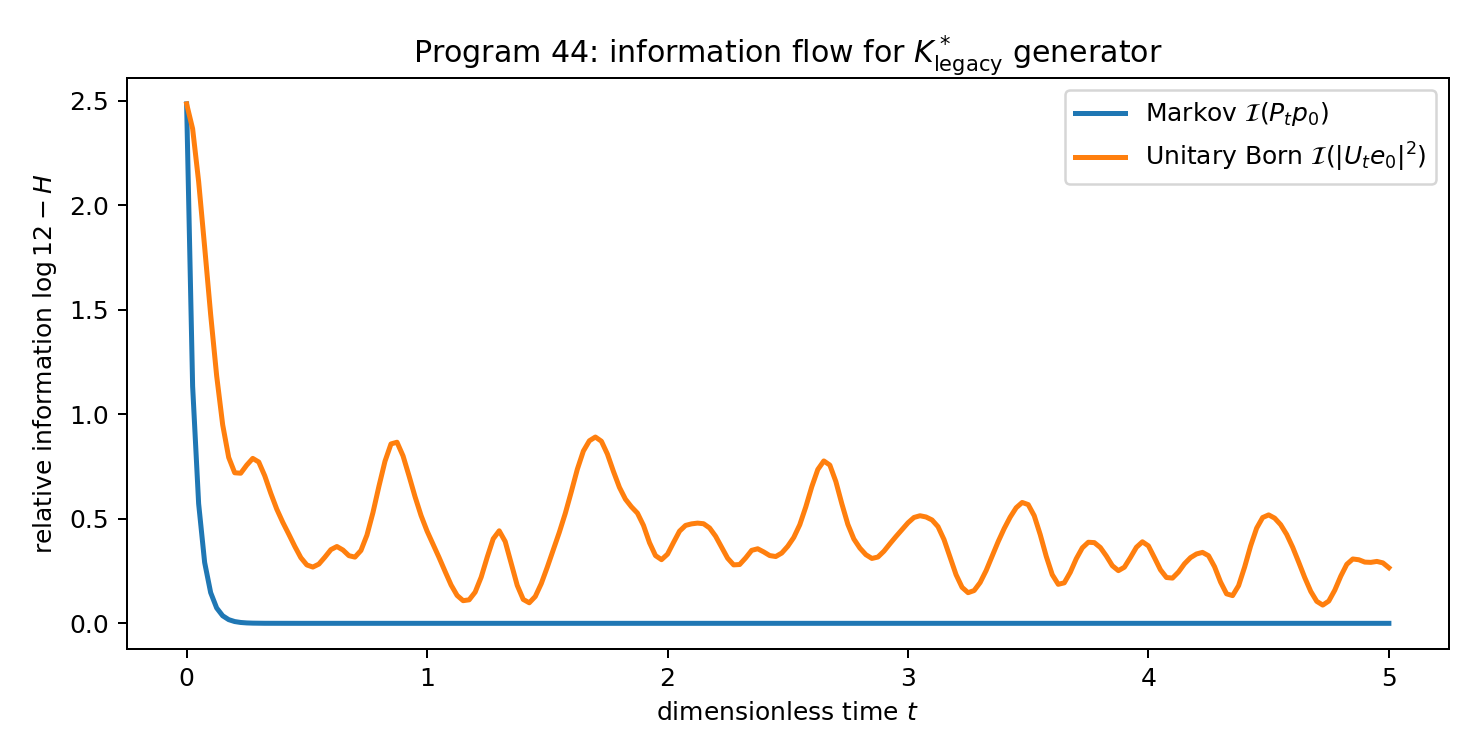
\includegraphics[width=0.92\textwidth]{FIN_Programs_41_50_Figures/program44_information_flow.png}
\caption{Relative information under Markov heat flow versus unitary Born populations for the abs-repaired historical \(K^*\) generator.}
\end{figure}


\textbf{\statusProven{}} Same spectrum, two temporal calculi; operator does not select which is physical time.

\section{Program 45 — environment recovery}

At dimensionless \(t=1\) for \(K^*_{\mathrm{Z12}}\) abs:

\begin{center}
\begingroup\small
\setlength{\tabcolsep}{3.5pt}
\renewcommand{\arraystretch}{1.16}
\begin{longtable}{@{}p{0.420\textwidth}p{0.420\textwidth}@{}}
\toprule
\textbf{Quantity} & \textbf{Value} \\
\midrule
\endhead
initial system relative info & \(2.485\) nats \\
final system relative info & \(0.135\) nats \\
apparent loss & \(2.350\) nats \\
pure-dilation mutual information \(I(S\!:\!E)\) & \(4.700\) nats \\
classical recovery fidelity & \(1\) \\
\bottomrule
\end{longtable}
\endgroup
\end{center}

\textbf{\statusProven{}} Apparent Markov loss is compatible with environmental transfer. Kernel alone does not source a physical bath.

\section{Program 46 — calibrated sign-reference emulator}

\(A\) from \(K^*\) is exactly inversion-even (residual \(0\)). External polarity \(\lambda=\pm 1\) changes double-slit detector response (difference \(\approx 0.049\) at site \(0\) for the scanned protocol). \textbf{\statusProven{}}

\textbf{\statusProven{}} External polarity is an apparatus/\allowbreak{}sector axiom, not a non-premise strict selector. QW-2191 remains open.

\section{Program 47 — influence-functional proxy}

Two-parameter Ohmic proxy for log-retention has residual \(\approx 0.45\) class and is post-hoc. \textbf{\statusModerate{}} No unique bath spectral density is derived from \(K^*\).

\section{Program 48 — feedback thermodynamic ledger}

Declared feedback matrix eigenvalues \(-0.8\pm 1.7i\), integrability defect \(\approx 0.905\), nonzero circulatory work proxy \(\approx 1.847\). \textbf{[Proven for the declared model]}

Stable non-gradient feedback can be added; it is not forced by \(K^*\) and does not yield unit-bearing \(L_{\mathrm{total}}\).

\section{Program 49 — process-tensor causal challenge}

Interventions change TV gaps between the \(K^*\) Markov process and a static spectral-gap mimic. Mean intervention margin on the scanned grid is small (\(\approx 0.0046\)) and model-dependent. \textbf{\statusModerate{}} Final-time fits alone are weak identifiers of causal structure.

\section{Program 50 — preregistered multi-size challenge}

Preregistered competitors: \(K^*_{\mathrm{hist}}\), \(K^*_{\mathrm{Z12}}\), classical legacy, rejected product, strict. On \(N=12,16,24\), cosine winners are always \textbf{strict} when strict is included.

On \(N=12\) cosines vs noisy strict target:

\begin{center}
\begingroup\small
\setlength{\tabcolsep}{3.5pt}
\renewcommand{\arraystretch}{1.16}
\begin{longtable}{@{}p{0.420\textwidth}p{0.420\textwidth}@{}}
\toprule
\textbf{Model} & \textbf{cosine} \\
\midrule
\endhead
strict & \(0.99997\) \\
rejected abs & \(0.936\) \\
\(K^*_{\mathrm{Z12}}\) abs & \(0.640\) \\
\(K^*_{\mathrm{hist}}\) abs & \(0.475\) \\
classical abs & \(0.454\) \\
\bottomrule
\end{longtable}
\endgroup
\end{center}

\begin{figure}[htbp]
\centering
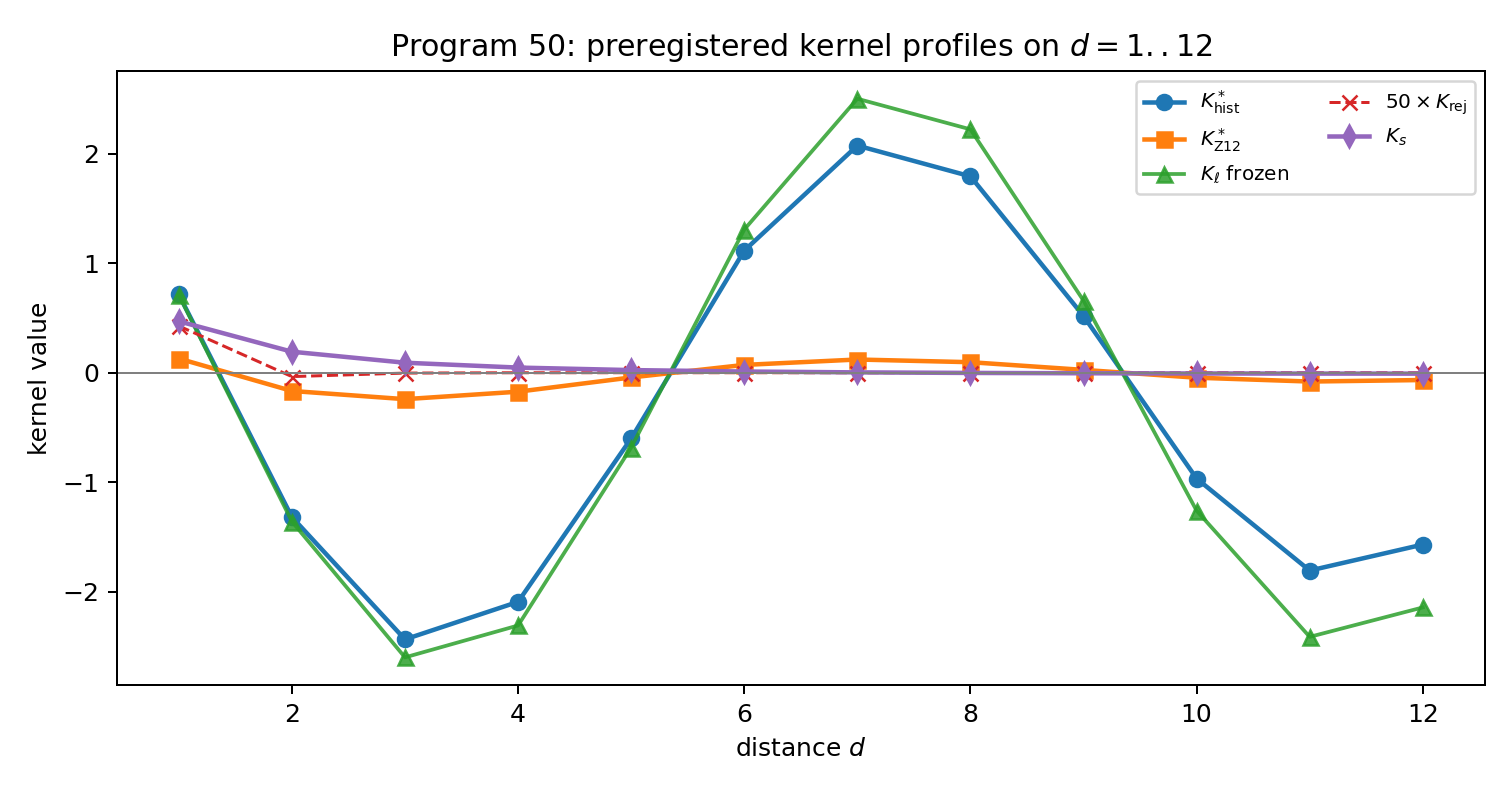
\includegraphics[width=0.92\textwidth]{FIN_Programs_41_50_Figures/program50_profiles.png}
\caption{Preregistered kernel profiles on \(d=1..12\): historical \(K^*\), \(\mathbb Z_{12}\) \(K^*\), classical frozen legacy, rejected product (scaled), and strict.}
\end{figure}


\textbf{\statusStrong{}} No legacy* form wins a multi-size challenge against strict. High cosine of the rejected product is an artifact of near-local tiny positive mass, not historical correctness.

\par\medskip\hrule\medskip

\chapter{Part IV — Leaf-cuts: units, selector, symmetry}

\section{\texorpdfstring{7. Does \(K^*\) fix dimensionlessness?}{7. Does K\textasciicircum{}* fix dimensionlessness?}}

\textbf{No. [Proven in the invariant-input sense of prior FAR audits; confirmed here.]}

\(K^*\) is a dimensionless radial profile. \(A\) and \(\beta\) are scale gauges of the same weight-zero class. Dual dynamics uses a dimensionless time parameter. No weight-one source \(S_+\), no \(\hbar_*\), no \((\ell_*,\tau_*)\) triad is exported.

Compatible with SUMMARY\_GROK.md: information is dimensionless; conversion axioms (CA) remain external unless a new source theorem appears.

\section{\texorpdfstring{8. Does \(K^*\) fix the selector /\allowbreak{} QW-2191?}{8. Does K\textasciicircum{}* fix the selector /\allowbreak{} QW-2191?}}

\textbf{No. [Proven for radial inversion-even data.]}

The Laplacian generated by radial \(K^*\) is invariant under \(x\mapsto -x\). Aut\((\mathbb Z_{12})\) still pairs opposite orientations. Program 46 shows polarity works only after an external apparatus sign is supplied.

\section{\texorpdfstring{9. Does \(K^*\) break symmetry internally?}{9. Does K\textasciicircum{}* break symmetry internally?}}

\textbf{Not as a non-premise strict source. [Proven /\allowbreak{} strong evidence.]}

The cosine supplies oscillatory structure and exact zeros at \(d=4/3+4n\), but those are phase-label data, not a theorem selecting one origin/\allowbreak{}polarity on the orientation torsor. Exact zeros are still not the integer sequence historically claimed.

\section{\texorpdfstring{10. What \(K^*\) \emph{does} improve}{10. What K\textasciicircum{}* *does* improve}}

\begin{center}
\begingroup\small
\setlength{\tabcolsep}{3.5pt}
\renewcommand{\arraystretch}{1.16}
\begin{longtable}{@{}p{0.420\textwidth}p{0.420\textwidth}@{}}
\toprule
\textbf{Aspect} & \textbf{Status under \(K^*\)} \\
\midrule
\endhead
Historical algebraic fidelity & improved vs product candidate \\
Path-sum asymptotics & corrected class \\
Dual dynamics after \(\lvert W\rvert\) repair & operationally usable \\
Markov CP-divisibility & yes after repair \\
Bridge to strict without extra maps & still no \\
Units /\allowbreak{} selector /\allowbreak{} ToE & still open \\
\bottomrule
\end{longtable}
\endgroup
\end{center}

\par\medskip\hrule\medskip

\chapter{Part V — Guardrail-compliant global verdict}

Under AGENTS.md:

\begin{itemize}
\item 
\(K_{\mathrm{legacy}}\) remains an \textbf{intermediate bridge kernel}, not a silent substitute for \(K_{\mathrm{strict}}\).

\item 
\(K^*\) is a cleaned intermediate of that legacy class, not a role-transfer theorem.

\item 
No promotion of \(L_{\mathrm{total}}\), bridge completion, or ToE.

\end{itemize}

Under SUMMARY\_GROK.md two-package language:

W0  informational nadsoliton + K* class (dimensionless) W1  CA: units (still missing) W2  SA: selector /\allowbreak{} polarity (still missing unless axiomatic) W3  effective dual dynamics conditioned on repairs and axioms

\textbf{Final status labels}

\begin{center}
\begingroup\small
\setlength{\tabcolsep}{3.5pt}
\renewcommand{\arraystretch}{1.16}
\begin{longtable}{@{}p{0.420\textwidth}p{0.420\textwidth}@{}}
\toprule
\textbf{Claim} & \textbf{Label} \\
\midrule
\endhead
Product \(K_{\mathrm{rej}}\) is historical reconstruction & \textbf{\statusRefuted{}} \\
Path-transformed class \(K^*\) matches historical intent algebra & \textbf{\statusProven{}} as class, not unique tuple \\
\(K^*\) supports dual dynamics after positivity repair & \textbf{\statusStrong{}} \\
\(K^*\) closes units leaf-cut & \textbf{\statusRefuted{}} \\
\(K^*\) closes selector leaf-cut & \textbf{\statusRefuted{}} \\
\(K^*\) alone completes legacy→strict & \textbf{\statusRefuted{}} \\
Programs 41–50 executed reproducibly & \textbf{\statusProven{}} for this suite \\
\bottomrule
\end{longtable}
\endgroup
\end{center}

\par\medskip\hrule\medskip

\chapter{Reproducibility}

\begin{center}
\begingroup\small
\setlength{\tabcolsep}{3.5pt}
\renewcommand{\arraystretch}{1.16}
\begin{longtable}{@{}p{0.420\textwidth}p{0.420\textwidth}@{}}
\toprule
\textbf{Artifact} & \textbf{Path} \\
\midrule
\endhead
Program 42a script & program\_42a\_legacy\_kernel\_reconstruction.py \\
Program 42a JSON & program\_42a\_legacy\_kernel\_reconstruction\_report.json \\
Programs 41–50 script & fin\_programs\_41\_50\_legacy\_star.py \\
Programs 41–50 JSON & FIN\_Programs\_41\_50\_Legacy\_Star\_Results.json \\
Figures & FIN\_Programs\_41\_50\_Figures/\allowbreak{} \\
This monograph & FIN\_Programs\_41\_50\_Legacy\_Star\_Monograph.md \\
\bottomrule
\end{longtable}
\endgroup
\end{center}

Seed: 20260719. Dependencies: NumPy, SciPy, Matplotlib.

\par\medskip\hrule\medskip

\chapter{Suggested citation}

Żuchowski, K. (2026). \emph{FIN Reconstructed Legacy Kernel: Program 42a Methodology Audit and Executed Programs 41–50 on \(K^*_{\mathrm{legacy}}\)} (FIN Research Supplement, Release 10.4; Version 1.0.0) [Preprint].


\clearpage
\chapter*{Archival note}
\addcontentsline{toc}{chapter}{Archival note}
Machine-readable results: \path{FIN_Programs_41_50_Legacy_Star_Results.json}, generated by \path{fin_programs_41_50_legacy_star.py}. Program~42a report: \path{program_42a_legacy_kernel_reconstruction_report.json}.

\medskip
\noindent\textbf{Suggested citation before DOI assignment:}

\.Zuchowski, K. (2026). \emph{FIN Reconstructed Legacy Kernel: Program 42a Methodology Audit and Executed Programs 41--50 on \(K^*_{\mathrm{legacy}}\)} (FIN Research Supplement, Release 10.4; Version 1.0.0) [Preprint].

\end{document}
